\section{Theorie}
\subsection{Der Zeeman-Effekt}
Verursacht durch den Elektronenspin $\vec{S}$ und den Bahndrehimpuls $\vec{L}$, hat jedes Energieniveau der Elektronen im Atom einen Gesamtdrehimpuls $\vec{J}$, welcher an ein magnetisches Moment koppelt:
\begin{equation}
  \vec{\mu}_J=\vec{\mu}_L+\vec{\mu}_S=-g_J\upmu_B\vec{J}
\end{equation}
bzw.
\begin{equation}
  ||\vec{\mu}_J||=-g_J\text{\mu}_B\sqrt{J(J+1)}\,.
\end{equation}
Hierbei ist $\mu_B$ das bohrsche Magneton und $g_J$ der Landé-Faktor
\begin{equation}
  g_J=1+\frac{J+(J+1)+S(S+1)-L(L+1)}{2J(J+1)}\,.
\end{equation}
Die magnetischen Momente $\mu_L$ und $\mu_S$ sind dabei gegeben durch
\begin{equation}
\vec{\mu}_L=-\mu_B\vec{L} \quad\quad\text{und}\quad\quad \vec{\mu}_S=-\text{g}_S\mu_B\vec{S}
\end{equation}
mit dem Landé-Faktor des freien Elektrons $\text{g}_S=2{,}00232$.
Wird das Atom zusätzlich von einem externen Magnetfeld $\vec{B}$ umgeben, so wechselwirkt dieses mit dem Elektron und es tritt eine Aufspaltung der Energieniveaus auf. Die Wechselwirkungsenergie ist dabei gegeben durch
\begin{equation}
  W=g_J\mu_BBM\,,
\end{equation}
wobei berücksichtigt wird, dass sich die zu $\vec{B}$ senkrechte Komponente zeitlich herausmittelt und die  Richtungsquantelung nur ganzzahlige Werte von $M \in [-J,J]$ zulässt. Es entsteht somit eine Aufspaltung jedes Energieniveaus in $2J+1$ Unterniveaus.
\subsection{Die Hyperfeinstrukturaufspaltung}
Neben der Feinstrukturaufspaltung, welche durch die Wechselwirkung der Ladung des Elektrons mit seinem Drehimpuls entsteht, ist bei echten Atomen auch noch der Kernspin zu beachten. Für schwache Magnetfelder tritt eine Kopplung von Kernspin $\vec{I}$ und Drehimpuls des Elektrons $\vec{J}$ zum Gesamtdrehimpuls des Atoms $\vec{F}=\vec{I}+\vec{J}$ auf. Das magnetische Moment des Kerns welches mit dem Kernspin gekoppelt ist, richtet sich im Magnetfeld des Elektrons gequantelt aus, wodurch es
eine Aufspaltung der Feinstrukturniveaus in $F \in [|I-J|,I+J]$ Hyperfeinstrukturniveaus gibt.
In einem schwachen Magnetfeld $B$ tritt zusätzlich der Zeeman-Effekt ein, welcher zu einer Aufspaltung der Hyperfeinstrukturniveaus in $2F+1$-Zeeman-Niveaus mit einer Energiedifferenz:
\begin{equation}
  E_{\text{HF}}=g_F\upmu_BB
\end{equation}
führt. Der relevante Landé-Faktor $g_F$ ist dabei gegeben durch:
\begin{equation}
  g_F=g_J\frac{F(F+1)+J(J+1)-I(I+1)}{2F(F+1)}\,.
\end{equation}
Das Termschema für den Grundzustand eines Alkaliatoms mit Kernspin $3/2$, wie es bei $^{87}$Rb der Fall ist, ist in Abb.\ref{Hyperfein} dargestellt.
\begin{figure}
  \centering
  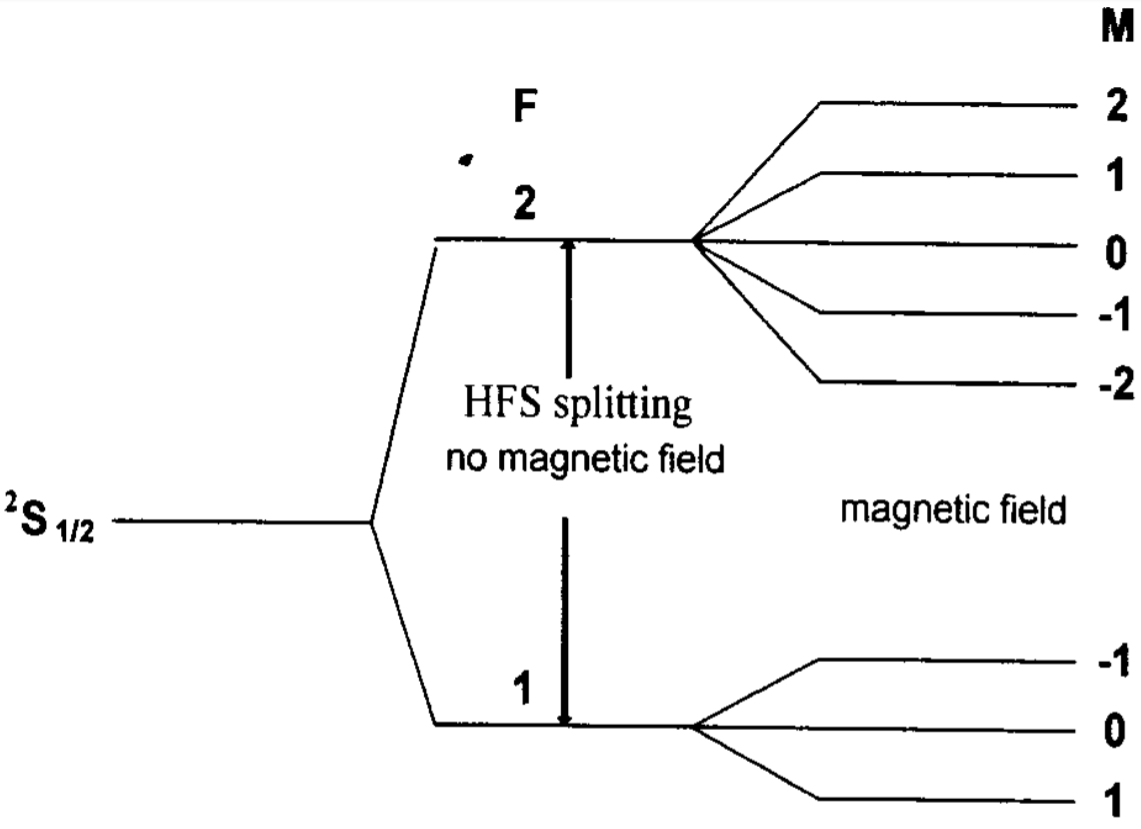
\includegraphics[scale=0.4]{Bilder/Hyperfein}
  \caption{Zustandsschema des Grundzustands eines Alkali-Atoms mit $I=3/2$\cite{Black}.}
  \label{Hyperfein}
\end{figure}
\subsection{Optisches Pumpen}
Für ein Atom, welches sich im thermischen Gleichgewicht mit seiner Umgebung befindet, sind die inneren Elektronenschalen gemäß des Pauli-Prinzips besetzt, während die Besetzung der Äußeren einer Boltzmann-Verteilung folgt. Das Verhältnis der Besetzungszahlen $N_i$ zweier Zustände ergibt sich somit durch
\begin{equation}
  \frac{N_2}{N_1}=\frac{g_2}{g_1}\frac{\exp\left(-\sfrac{W_2}{\symup{k_B}T}\right)}{\exp(-\sfrac{W_1}{\symup{k_B}T})}\,,
  \label{eq:thermisch}
\end{equation}
wobei $W_i$ die Energie des $i$-ten Zustands, $T$ die Temperatur und $g_i$ statistische Gewichte sind.\\
Die gezielte Erzeugung einer Abweichung der Besetzungszahlen vom thermischen Gleichgewicht wird als optisches Pumpen bezeichnet, wobei bei ausreichendem Pumpen auch eine Besetzungsinversion erzeugt werden kann. Der in diesem Versuch genutzte Pumpprozess wird im Folgenden beschrieben.\\
Der Pumpprozess beginnt mit dem Einstrahlen von zirkular polarisiertem D$_1$-Licht auf das Rubidium. Hierbei werden Elektronen vom Grundzustand $^2$S$_{1/2}$ in den ersten angeregten Zustand $^2$P$_{1/2}$ gehoben, wobei wegen der Polarisation der Photonen die Auswahlregel $\Delta M=\pm1$ für Übergänge befolgt werden muss. Das Vorzeichen der Auswahlregel
\begin{wrapfigure}{r}{0.55\textwidth}
  \centering
  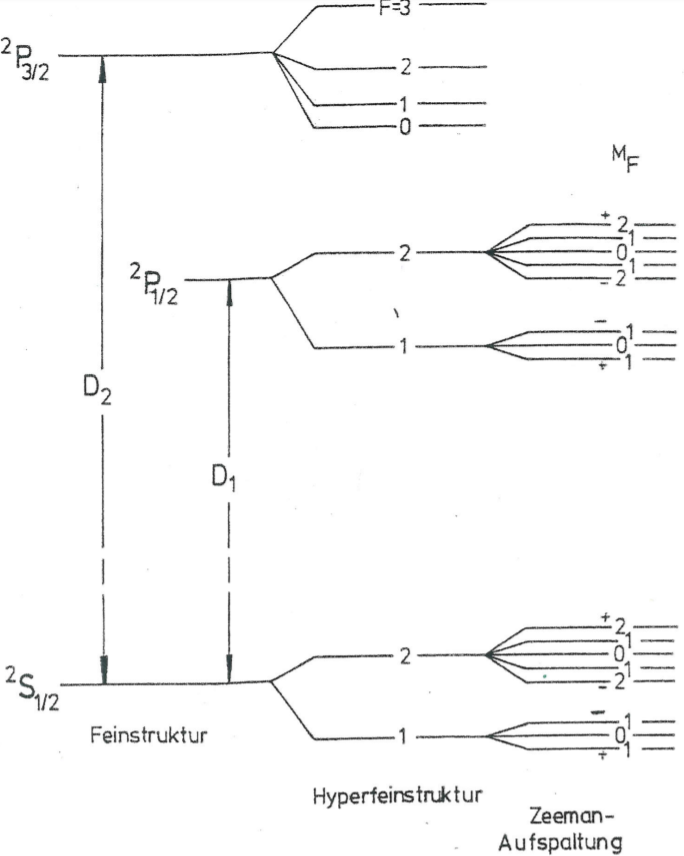
\includegraphics[width=0.55\textwidth]{Bilder/D1}
  \caption{Darstellung der D$_1$ und D$_2$ Übergänge in $^{87}$Rb \cite{D1}.}
\end{wrapfigure}
 hängt dabei von der Polarisationsrichtung ab, für rechtszirkularpolarisiertes Licht gilt $\Delta M=1$, diese Übergänge werden $\sigma^+$ genannt. Übergänge mit linkszirkularpolarisiertem Licht haben $\Delta M=-1$ und werden $\sigma^-$ genannt.
Für linearpolarisiertes Licht finden $\pi$-Übergänge statt, welche $\Delta M=0$ haben. Handelt es sich bei der D$_1$-Strahlung nun um rechtszirkularpolarisiertes Licht werden wegen der Auswahlregeln alle Grundzustandniveaus angeregt, bis auf der, welcher aufgrund von $\Delta M=1$ keine erlaubten Übergänge hat. Vom angeregten Zustand fallen die Elektronen durch Emission wieder in den Grundzustand zurück, wobei hierbei Übergänge in alle Grundzustandniveaus erlaubt sind. Es werden somit nach hinreichender Zeit die Elektronen in den Zustand gepumpt, dessen Anregung verboten ist.
Bei den Emissionsprozessen muss im Allgemeinen zwischen spontaner und induzierter Emission unterschieden werden. Für induzierte Emission wird ein Photon benötigt, welches dieselbe Energie wie die Energielücke zwischen den Zuständen hat. Das angeregte Elektron fällt daraufhin in den niedriegeren Zustand ab und sendet dabei ein Photon aus, welches dieselbe Energie, Phase und Ausbreitungsrichtung wie das induzierende Photon hat.
Es ist anzumerken, dass die Wahrscheinlichkeit für spontane Emission mit $\nu^3$ von der Frequenz des emittierten Photons abhängt, weswegen in diesem Pumpprozess die spontanen Übergänge zwischen den Zeeman-Niveaus nicht relevant sind.
\begin{figure}
  \centering
  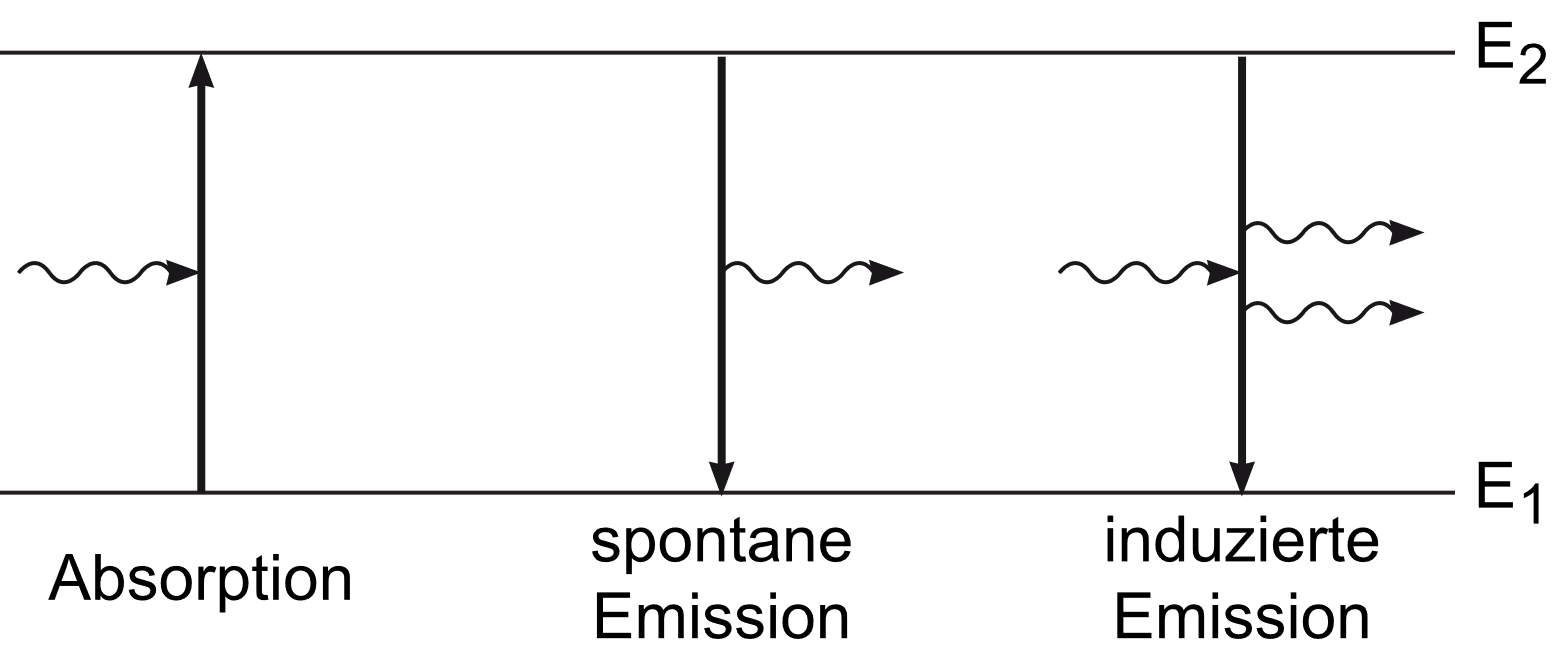
\includegraphics[width=0.5\textwidth]{Bilder/Emission}
  \caption{Schematische Darstellung von Absorption, spontaner Emission und induzierter Emission.\cite{Emission}}
\end{figure}
Wenn durch das optische Pumpen eine Besetzungsinversion erreicht ist, lässt sich diese durch ein angelegtes hochfrequentes RF-Feld wieder aufheben. Wenn das RF-Feld die Resonanzfrequenz der Zeeman-Niveauübergänge
\begin{equation}
  \nu_{\text{res}}=g_F\mu_0B/\text{h}
\end{equation}
annimmt, findet induzierte Emission statt, wodurch die Besetzungsinversion zerfällt.\\
Die Erzeugung einer Besetzungsinversion und deren Aufhebung wirkt sich auf die Transparenz von Rubidiumdampf aus. Da im thermischen Gleichgewicht ein großer Teil der Photonen zur Anregung absorbiert wird ist der Dampf zunächst nicht transparent, da Atome mit gepumpten Elektronen jedoch nicht von den Photonen angeregt werden könne nicht die Zahl der Absorptionen ab. Bei vollständiger Besetzungsinversion ist der Rubidiumdampf schließlich transparent. Die Absorptionsrate lässt sich durch das RF-Feld dann erneut erhöhen. Der Verlauf der Transparenz einer Zelle welche mit Rubidiumdampf gefüllt ist während eines solchen Pump-RF-Kreislaufs ist in Abb.\ref{Kreislauf} dargestellt.  In der Darstellung wird die Feldstärke des RF-Felds variiert, sodass sie den Resonanzfall überquert
\begin{figure}
  \centering
  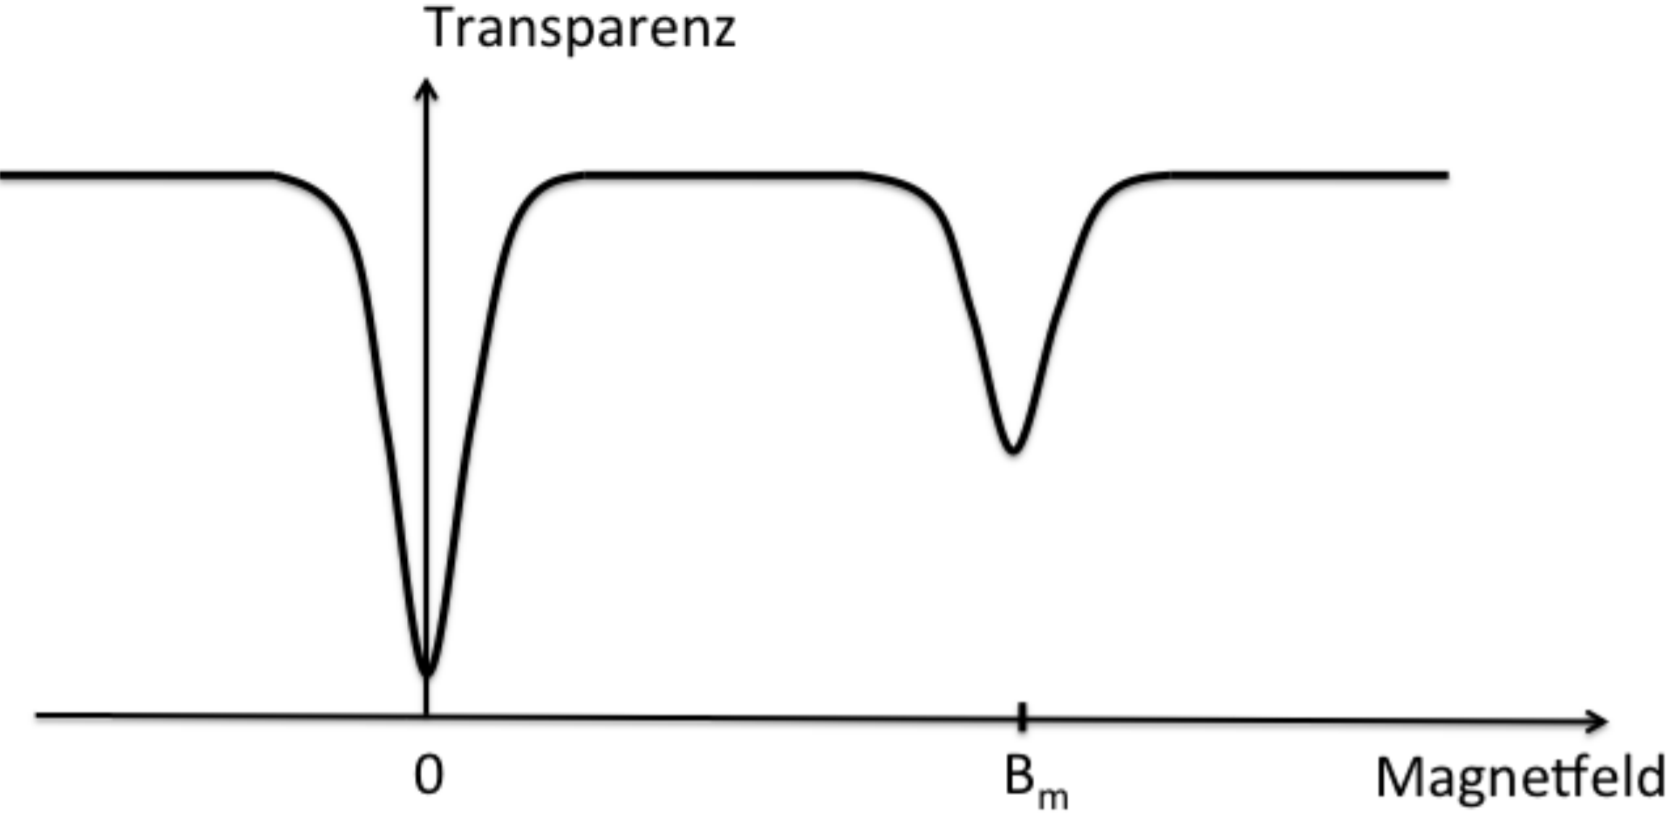
\includegraphics[width=0.5\textwidth]{Bilder/Beispiel}
  \caption{Schematische Darstellungs der Transparenzänderung einer Rubidiumdampfzelle bei Änderung der Feldstärke eines RF-Feldes \cite{Anleitung}.}
  \label{Kreislauf}
\end{figure}.
\subsection{Der quadratische Zeeman-Effekt}
In Anwesenheit starker Magnetfelder erfordert die Beschreibung des Zeeman-Effekts quadratische Terme in der Berechnung. Die Energiedifferenz der Niveaus ist dann gegeben durch:
\begin{equation}
  W = g_F\mu_\text{0}B+g^2_F\mu^2_\text{0}B^2\frac{1-2M_F}{\upDelta E_\text{Hyp}}
  \label{eq:quadratisch}
\end{equation}
mit der Energiedifferenz der Hyperfeinstrukturniveaus $\upDelta E_\text{Hyp}$.
\subsection{Transiente Effekte}
Transiente Effekte treten auf, wenn das RF-Feld so eingestellt ist, dass es in Resonanz mit dem System geschaltet ist und dann schnell ein- und abgeschaltet wird. Die Resonanzfrequenz $\omega_0$ ist dabei gegeben durch:
\begin{equation}
\omega_0=2\pi\nu_0=g_F\frac{\upmu_0}{\hbar}B_0=g_F\gamma B_0\,,
\end{equation}
wobei $\gamma$ als gyromagnetisches Verhätnis bezeichnet wird. Im schnell ändernden Magnetfeld präzedieren die Spins mit der Larmor-Frequenz $\nu=\gamma\text{B}_\text{RF}$ um $\text{B}_\text{RF}=\text{B}_\text{eff}$. Da die Resonanz von den Landé-Faktoren der Isotope abhängig ist, lässt sich durch die Periodendauern T der Präzessionen das Verhältnis der Isotope bestimmen:
\begin{equation}
  \frac{T_{87}}{T_{85}}=\frac{\gamma_{85}}{\gamma_{87}}\,.
\end{equation}
